\documentclass[12pt]{article}
%--------------------   start of the 'preamble'
%
\usepackage{graphicx,amssymb,amstext,amsmath,color}
\usepackage[margin=2cm]{geometry}
\usepackage{abstract}
\usepackage{setspace}
\usepackage[footnotesize,bf]{caption}

% TABLE
\usepackage{multicol,hhline,colortbl,multirow}
\usepackage{braket}
\usepackage{siunitx}
\usepackage{hyperref}
\usepackage{authblk}
\usepackage{siunitx}
\usepackage{mathrsfs}
%%\usepackage[sort&compress]{natbib}
%%\bibpunct{(}{)}{,}{a}{, }{;}
%
\usepackage[sort&compress]{natbib}
\bibpunct{[}{]}{,}{s}{}{;}


\definecolor{gray}{gray}{0.8}
\def\mobunits{\square\centi\meter\per\volt\per\second}
\def\gcm{\gram\per\cubic\centi\meter}
\def\ccg{\cellcolor{gray}}

\renewcommand{\labelitemii}{$\circ$}
\renewcommand{\bibname}{References}


\title{MorphCT Results - Voronoi Neighbour Analysis}
\author{Matthew Jones}
\date{\today}

\begin{document}
\maketitle

\section{Jobs run using the new Voronoi cell neighbourlist calculation}

\textcolor{red}{NOTE, In order to test the full pipeline after the recent changes to MorphCT, these jobs have been re-fine-grained (using the same MD parameters) so are somewhat different morphologies to previously.
I didn't think this would make much of a difference, but it seems like it might.
We need to perform a sensitivity analysis by comparing these results to the previously fine-grained morphologies but using the new neighbourlist calculation, to see how sensitive our results are to the fine-graining process..
Unfortunately, I have had some issues running the previous morphologies through the new Voronoi cell neighbourlist calculation, so these are delayed but should hopefully be completed by the end of the week.}

\begin{center}
\begin{tabular}{| c | c | c | c | c | c | c |}
\hline
\rule{0pt}{2.5ex} 
\multirow{2}{*}{\textbf{ID}}&\multirow{2}{*}{\textbf{Simulation Name}}&\textbf{Density}&\textbf{Anisotropy}&\textbf{Anisotropy}&\textbf{Mobility}&\textbf{Intra-}\\
                            &&(\SI{}{\gcm})&(Arb. U.)&(Shape)&(\SI{}{\mobunits})&\textbf{\%}\\
\hhline{|=======|}
\textbf{\ccg1}&\rule{0pt}{2.5ex}\ccg p1-L15-f0.0-P0.1-T1.5-e0.5&\ccg 1.676&\ccg 0.0676&\ccg ---&\ccg1.17$\times 10^{1}$&\ccg12.53\%\\
\textbf{2}&\rule{0pt}{2.5ex}p1-L15-f0.0-P0.1-T1.75-e0.5&1.061&0.0065&Spherical&3.48$\times 10^{-1}$&17.59\%\\
\textbf{\ccg3}&\rule{0pt}{2.5ex}\ccg p1-L15-f0.0-P0.1-T2.0-e0.5&\ccg 0.892&\ccg 0.0026&\ccg Spherical&\ccg4.46$\times 10^{-1}$&\ccg17.58\%\\
\textbf{4}&\rule{0pt}{2.5ex}p1-L15-f0.0-P0.1-T2.25-e0.5&0.787&0.0044&Spherical&5.52$\times 10^{-1}$&17.83\%\\
\textbf{\ccg5}&\rule{0pt}{2.5ex}\ccg p1-L15-f0.0-P0.1-T2.5-e0.5&\ccg 0.685&\ccg 0.0041&\ccg Spherical&\ccg4.03$\times 10^{-1}$&\ccg18.00\%\\
\hhline{|=======|}
\textbf{\ccg6}&\rule{0pt}{2.5ex}\ccg 0001\_withImages&\ccg 1.061&\ccg 0.0059&\ccg Spherical&\ccg2.65$\times 10^{-1}$&\ccg17.46\%\\
\textbf{7}&\rule{0pt}{2.5ex}0005\_withImages&1.336&0.0077&Spherical&4.68$\times 10^{-2}$&13.34\%\\
\textbf{\ccg8}&\rule{0pt}{2.5ex}\ccg 0010\_withImages&\ccg 1.345&\ccg 0.0063&\ccg Spherical&\ccg7.50$\times 10^{-1}$&\ccg13.73\%\\
\textbf{9}&\rule{0pt}{2.5ex}0020\_withImages&1.428&0.0137&Spherical&1.22$\times 10^{0}$&13.23\%\\
\textbf{\ccg10}&\rule{0pt}{2.5ex}\ccg 0040\_withImages&\ccg 1.450&\ccg 0.0077&\ccg Spherical&\ccg7.92$\times 10^{-2}$&\ccg13.78\%\\
\textbf{11}&\rule{0pt}{2.5ex}0100\_withImages&1.510&0.0228&Spherical&4.33$\times 10^{0}$&12.89\%\\
\textbf{\ccg12}&\rule{0pt}{2.5ex}\ccg 0200\_withImages&\ccg 1.554&\ccg 0.0721&\ccg Ellipsoid&\ccg4.94$\times 10^{0}$&\ccg12.74\%\\
\textbf{13}&\rule{0pt}{2.5ex}0300\_withImages&1.593&0.1041&Disk&6.44$\times 10^{0}$&12.61\%\\
\textbf{\ccg14}&\rule{0pt}{2.5ex}\ccg 0500\_withImages&\ccg 1.638&\ccg 0.1186&\ccg Disk&\ccg9.26$\times 10^{0}$&\ccg12.55\%\\
\textbf{15}&\rule{0pt}{2.5ex}1000\_withImages&1.662&0.0957&Disk&9.11$\times 10^{0}$&12.49\%\\
\hhline{-------}
\end{tabular}\label{table:mob}
\captionof{table}{The results from the new data given a snapshot of the pristine P3HT morphology at a given snapshot corresponding to simulation time, $\tau$.}
\end{center}

\begin{figure}[h!]\centering
	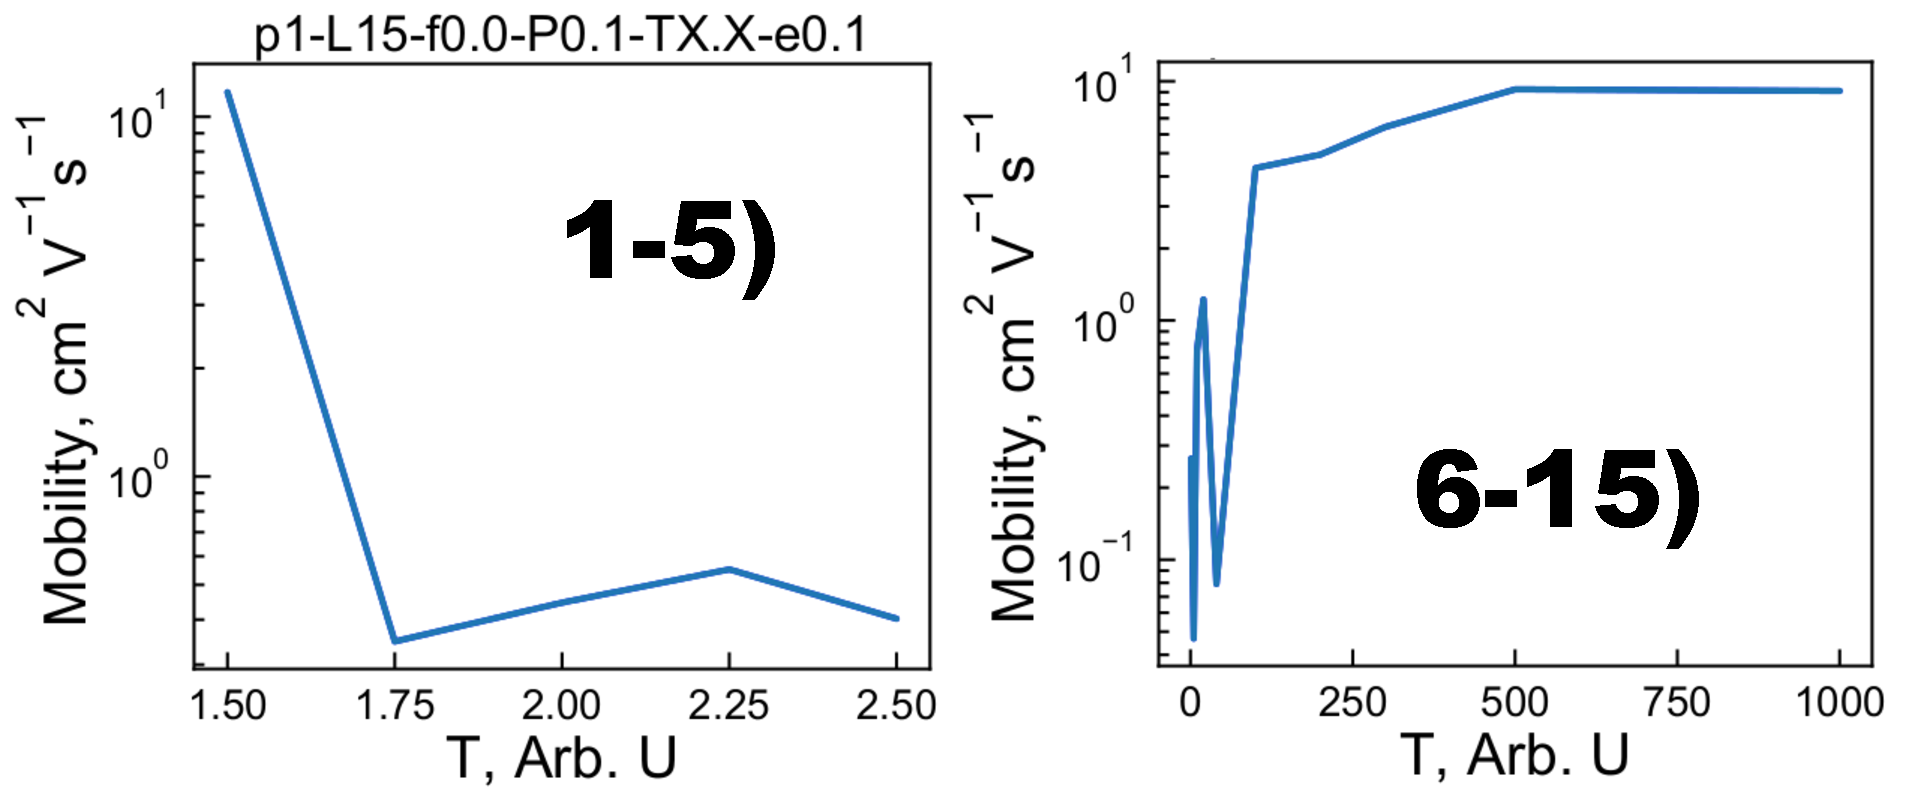
\includegraphics[width=\textwidth]{Figures/mobilityHole.pdf}
    \caption{The mobility trend observed as a function of increasing dimensionless evolution time}
	\label{fig:MSD}
\end{figure}

Representative Values From Literature:
\begin{itemize}
    \item{Density: \SI{1.10}{\gcm}\cite{Newbloom2012a}}
\item{Mobility: \SI{1E-5}{} - \SI{1E-3}{\mobunits}\cite{Ballantyne2008b,Mauer2010,Pandey2000,Kim2006}}
\end{itemize}

\clearpage

\subsection{3D Carrier Network}

\begin{figure}[h!]\centering
	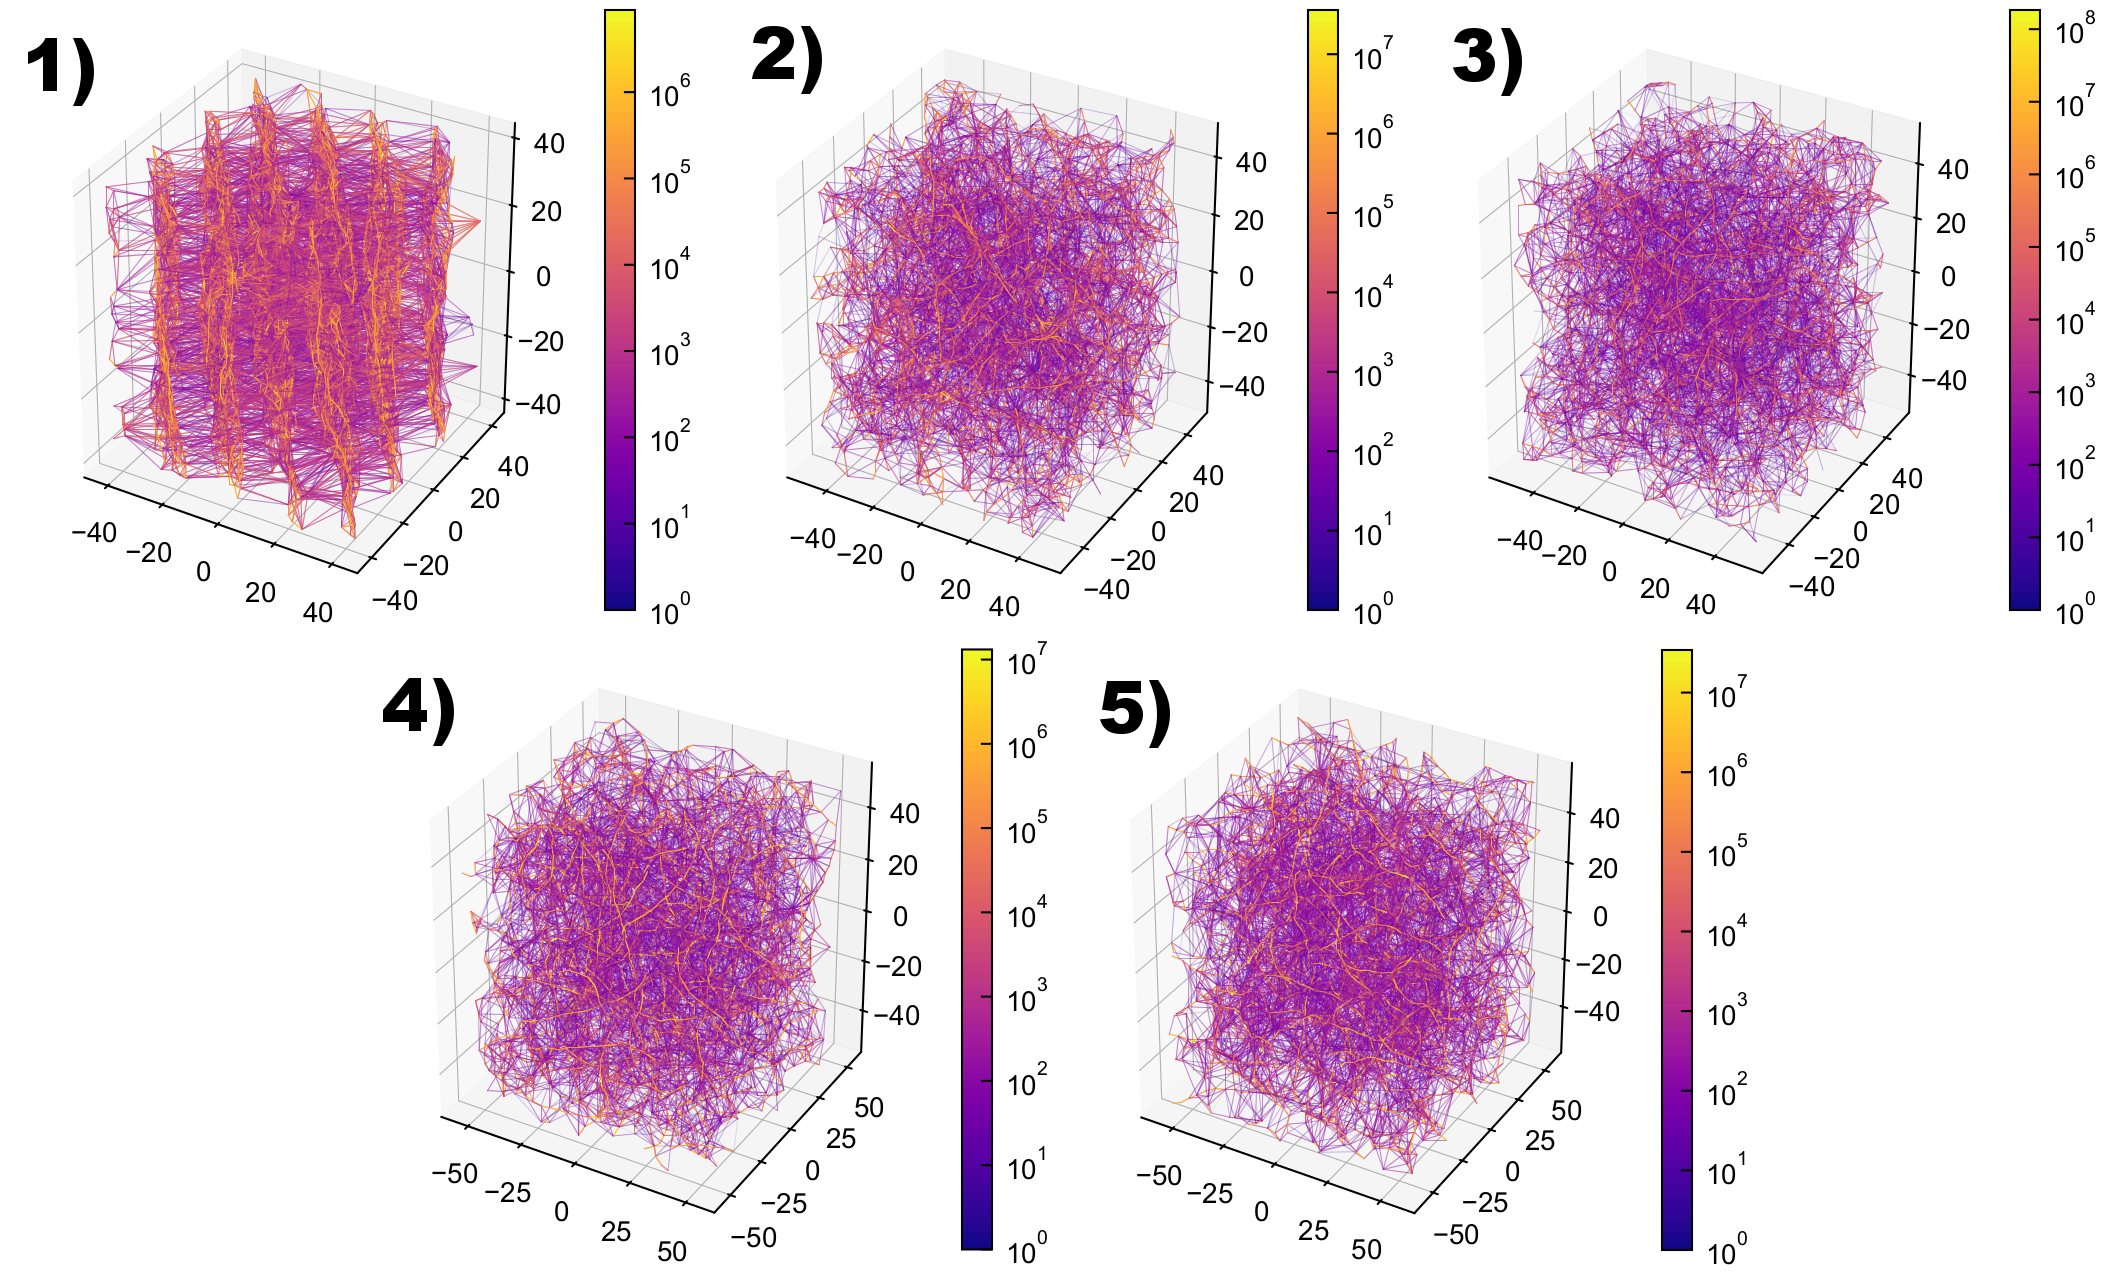
\includegraphics[width=\textwidth]{Figures/3dHole.png}
    \caption{The 3D heatmap of charge transport routes within the morphologies \textbf{1} - \textbf{5}.
    More yellow routes describe commonly accessed hops between pairs of chromophores, whereas more purple routes are less widely used in the KMC simulations.
    Each node therefore represents the location of a single chromophore.
The intensity value for the route is currently taken to be \texttt{I $=$ np.log10(freq) $/$ np.log10(max\_freq)}.}
	\label{fig:3dNetwork}
\end{figure}


\begin{figure}[h!]\centering
	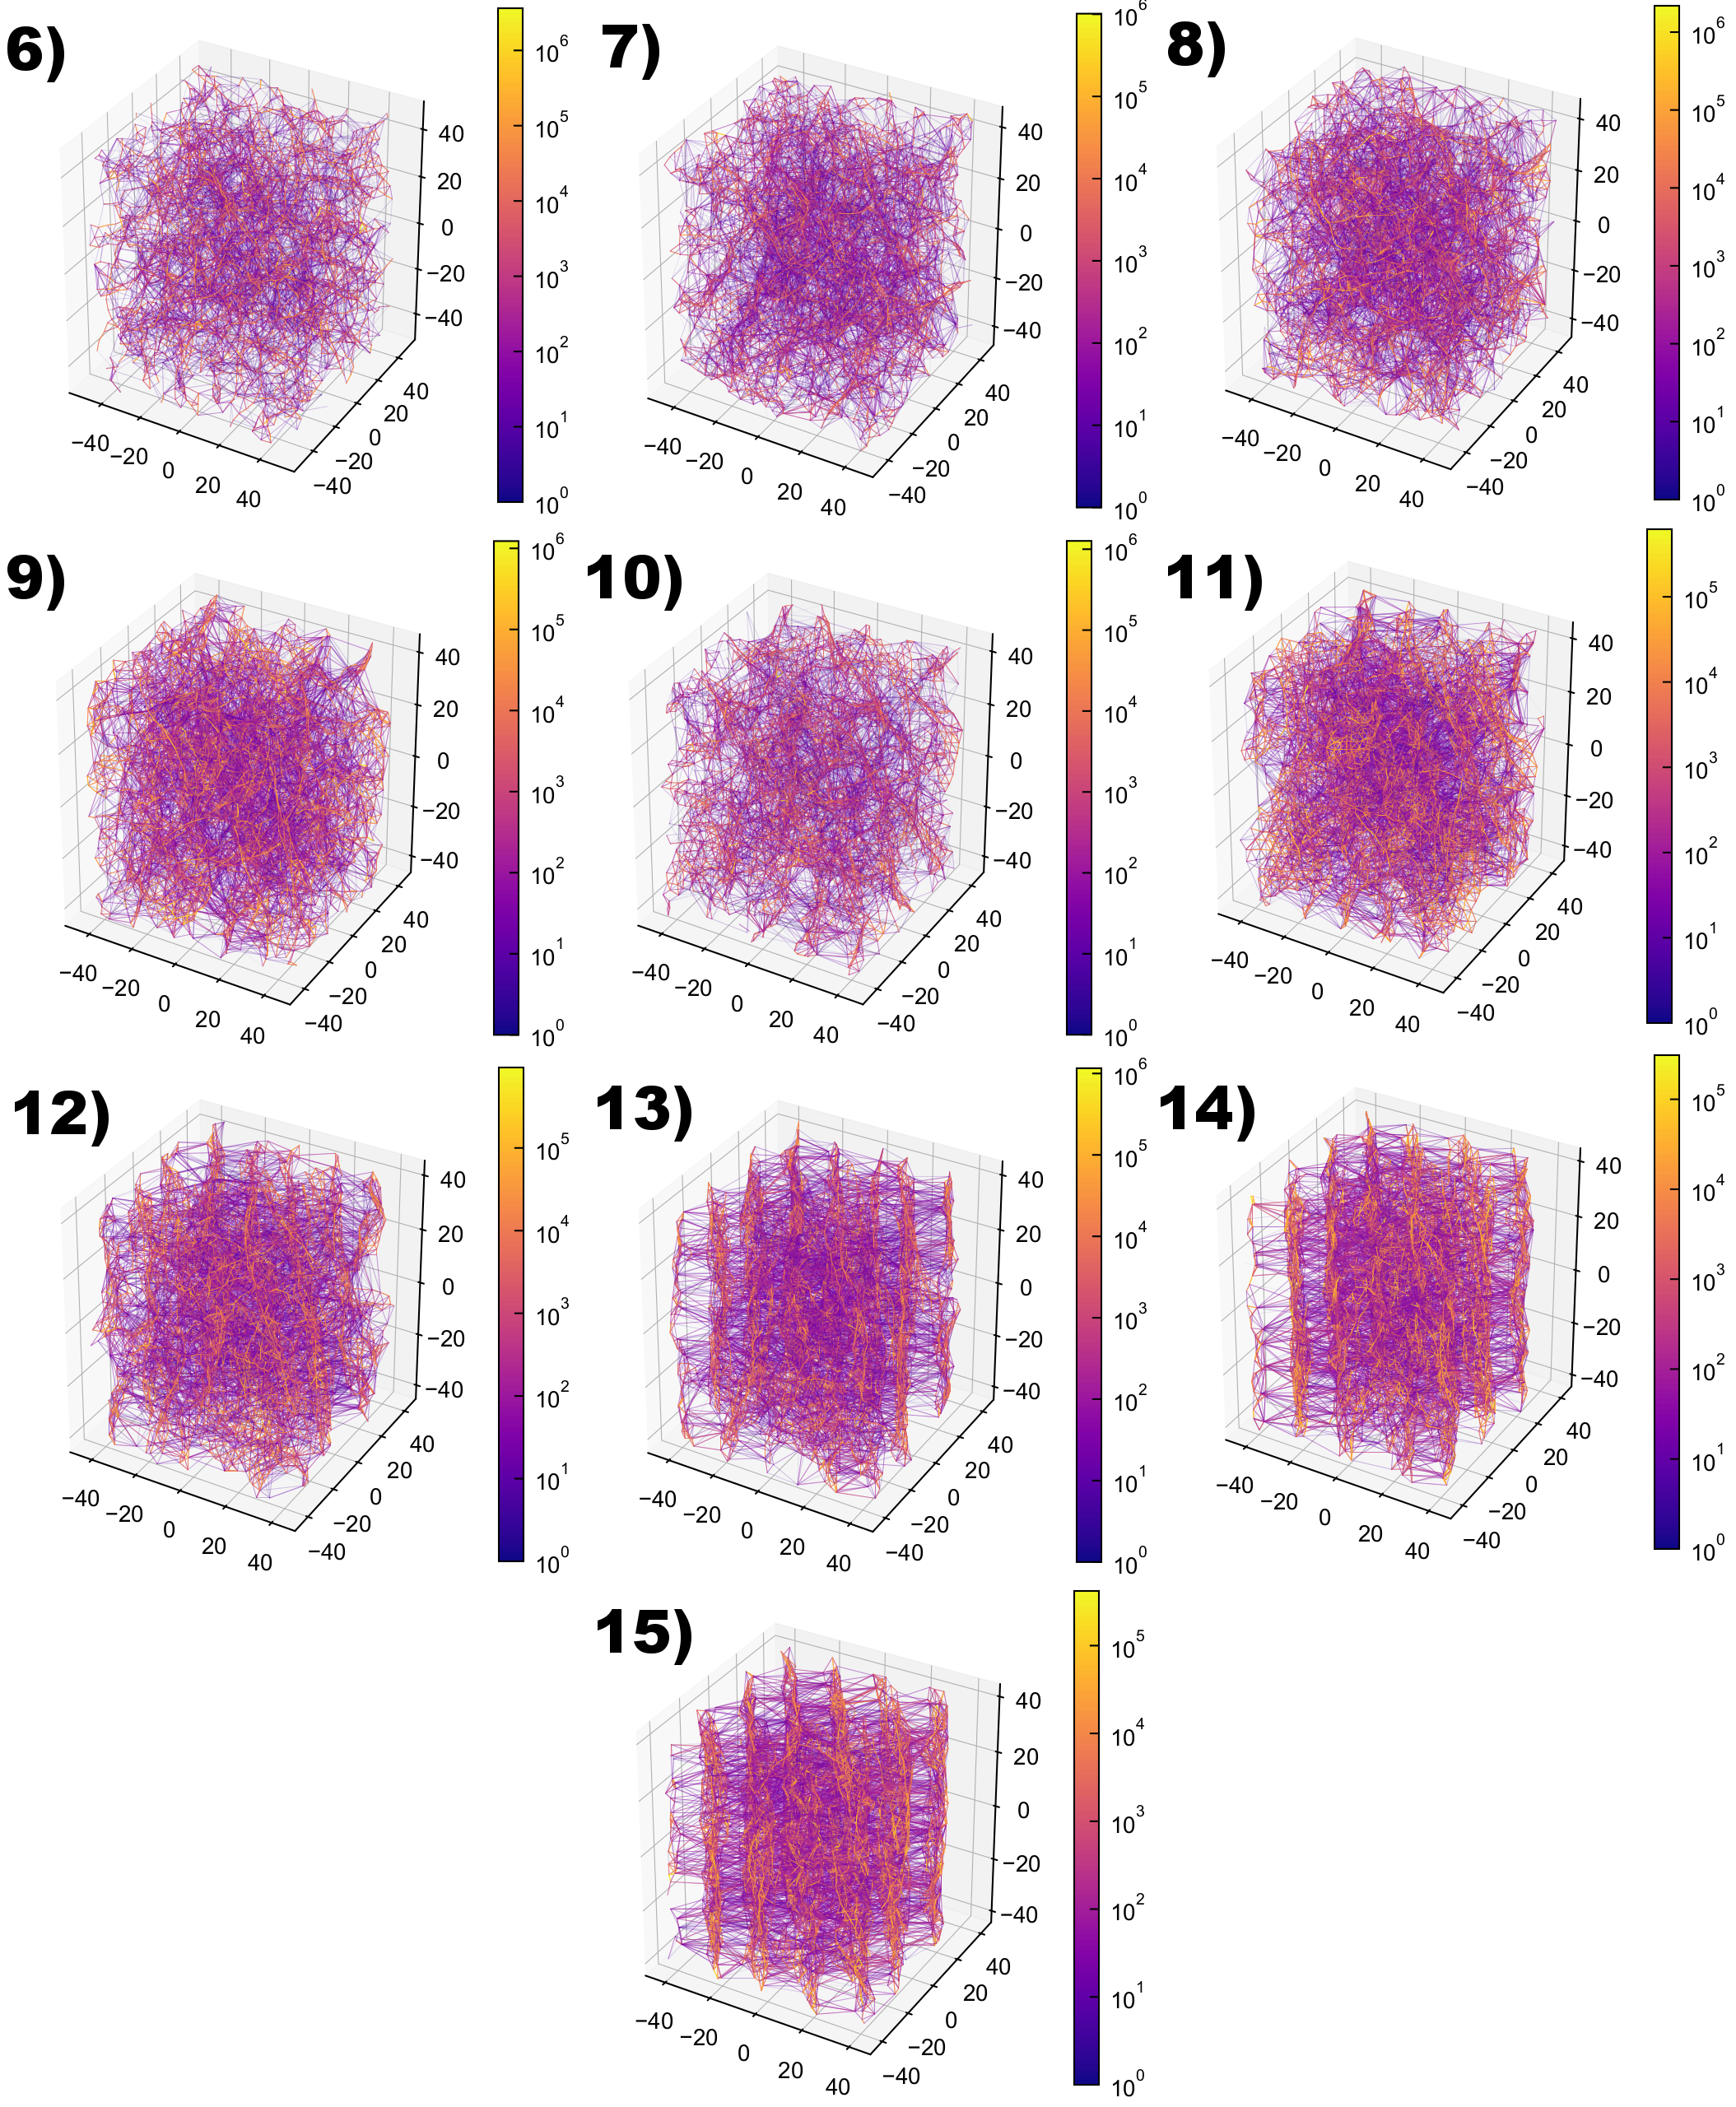
\includegraphics[width=\textwidth]{Figures/3dHoleFrame.png}
    \caption{The 3D heatmap of charge transport routes within the morphologies \textbf{6} - \textbf{15}.
    More yellow routes describe commonly accessed hops between pairs of chromophores, whereas more purple routes are less widely used in the KMC simulations.
    Each node therefore represents the location of a single chromophore.
The intensity value for the route is currently taken to be \texttt{I $=$ np.log10(freq) $/$ np.log10(max\_freq)}.}
	\label{fig:3dNetwork}
\end{figure}


\clearpage
\subsection{Anisotropies}


\begin{figure}[h!]\centering
	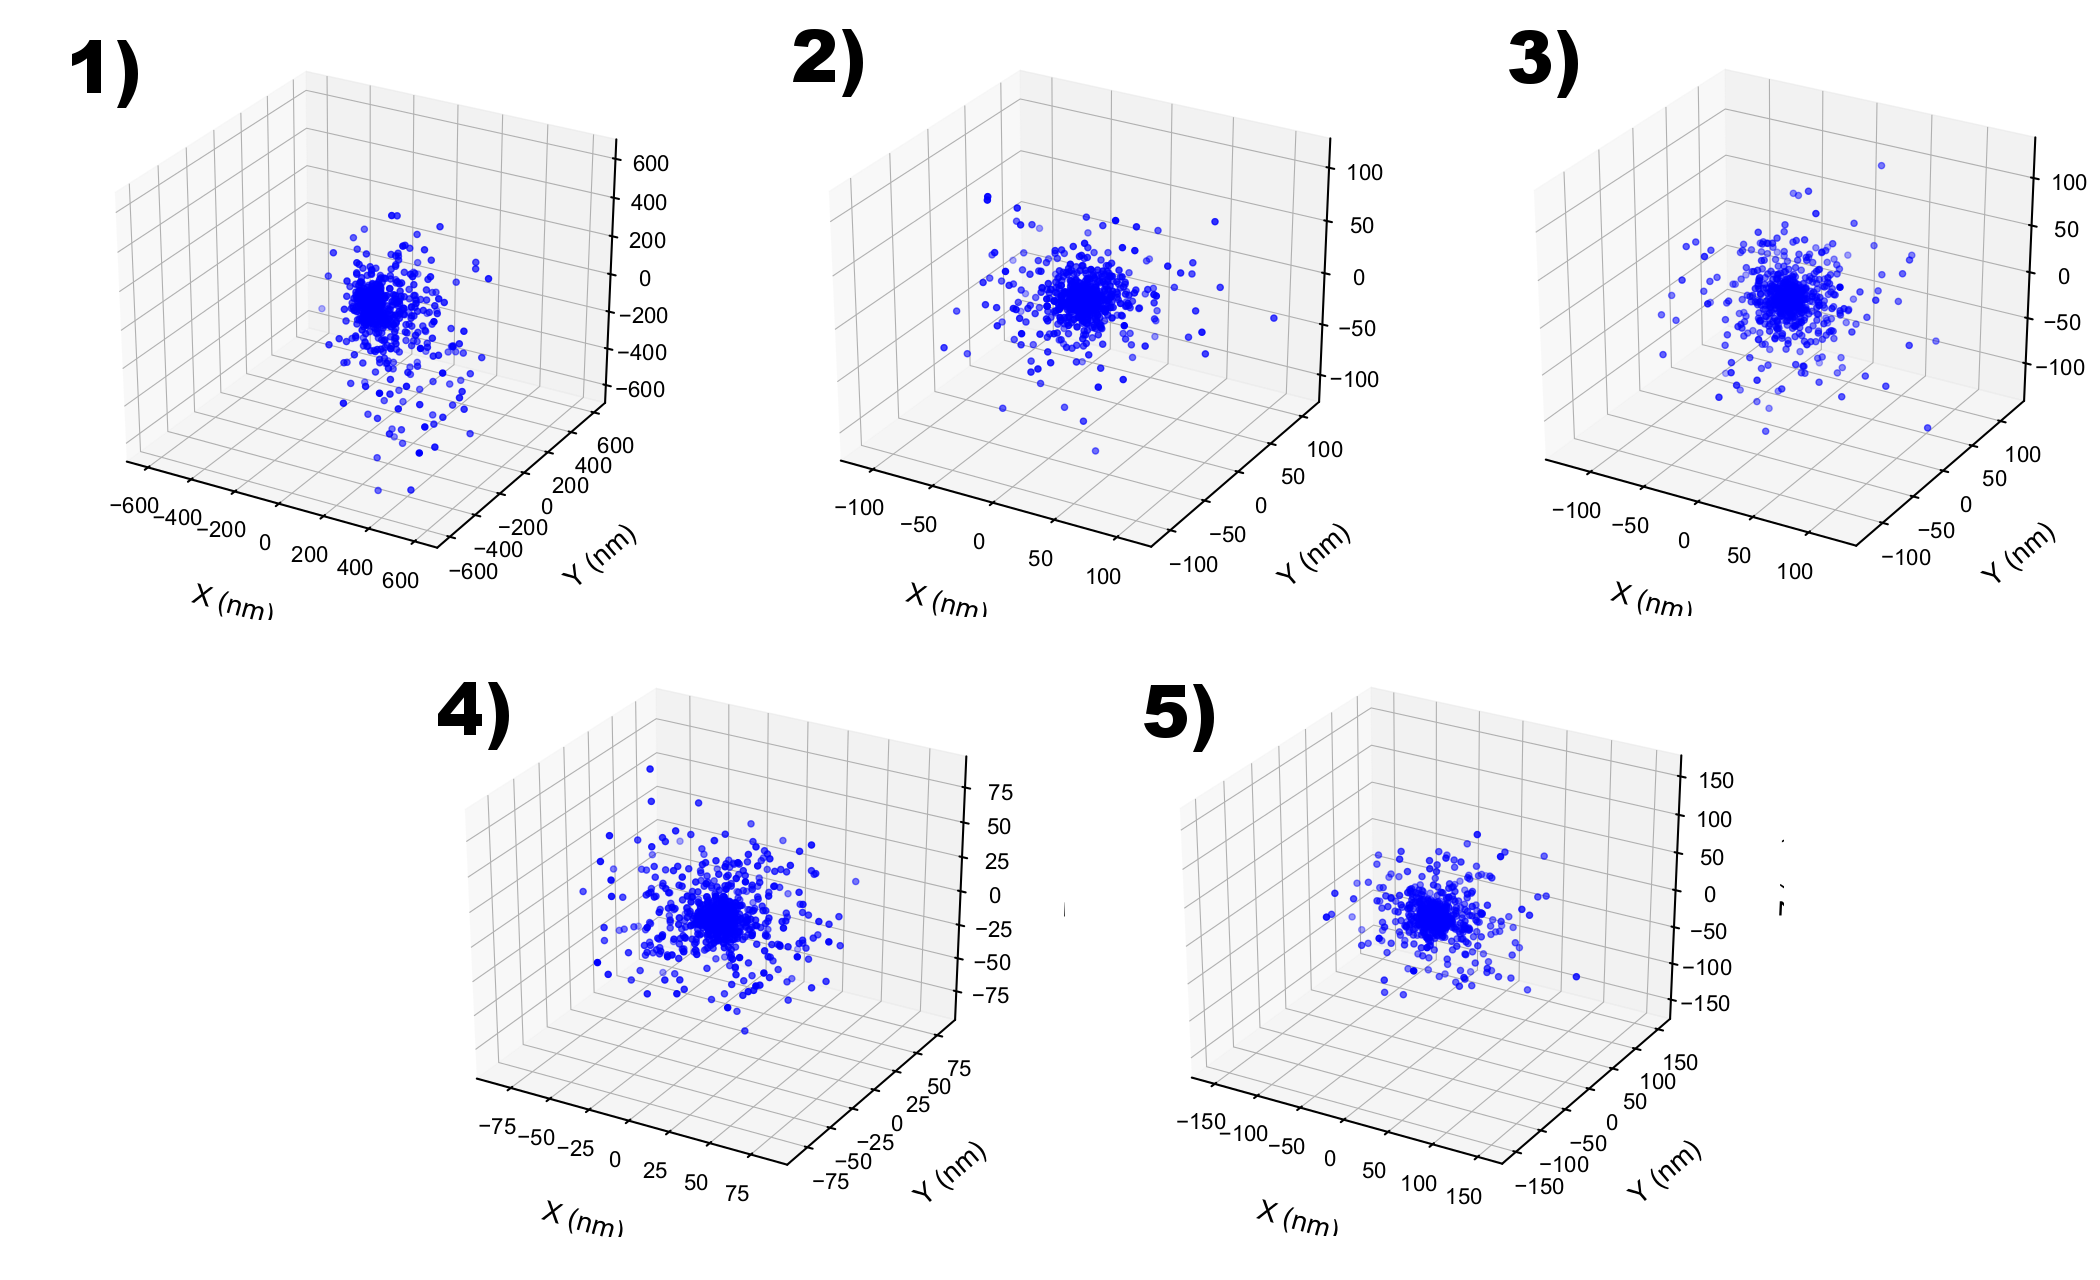
\includegraphics[width=\textwidth]{Figures/anisotropyHole.png}
    \caption{The periodic anisotropies of the carrier transport within the morphologies \textbf{1} - \textbf{5}.}
	\label{fig:MSD}
\end{figure}

\begin{figure}[h!]\centering
	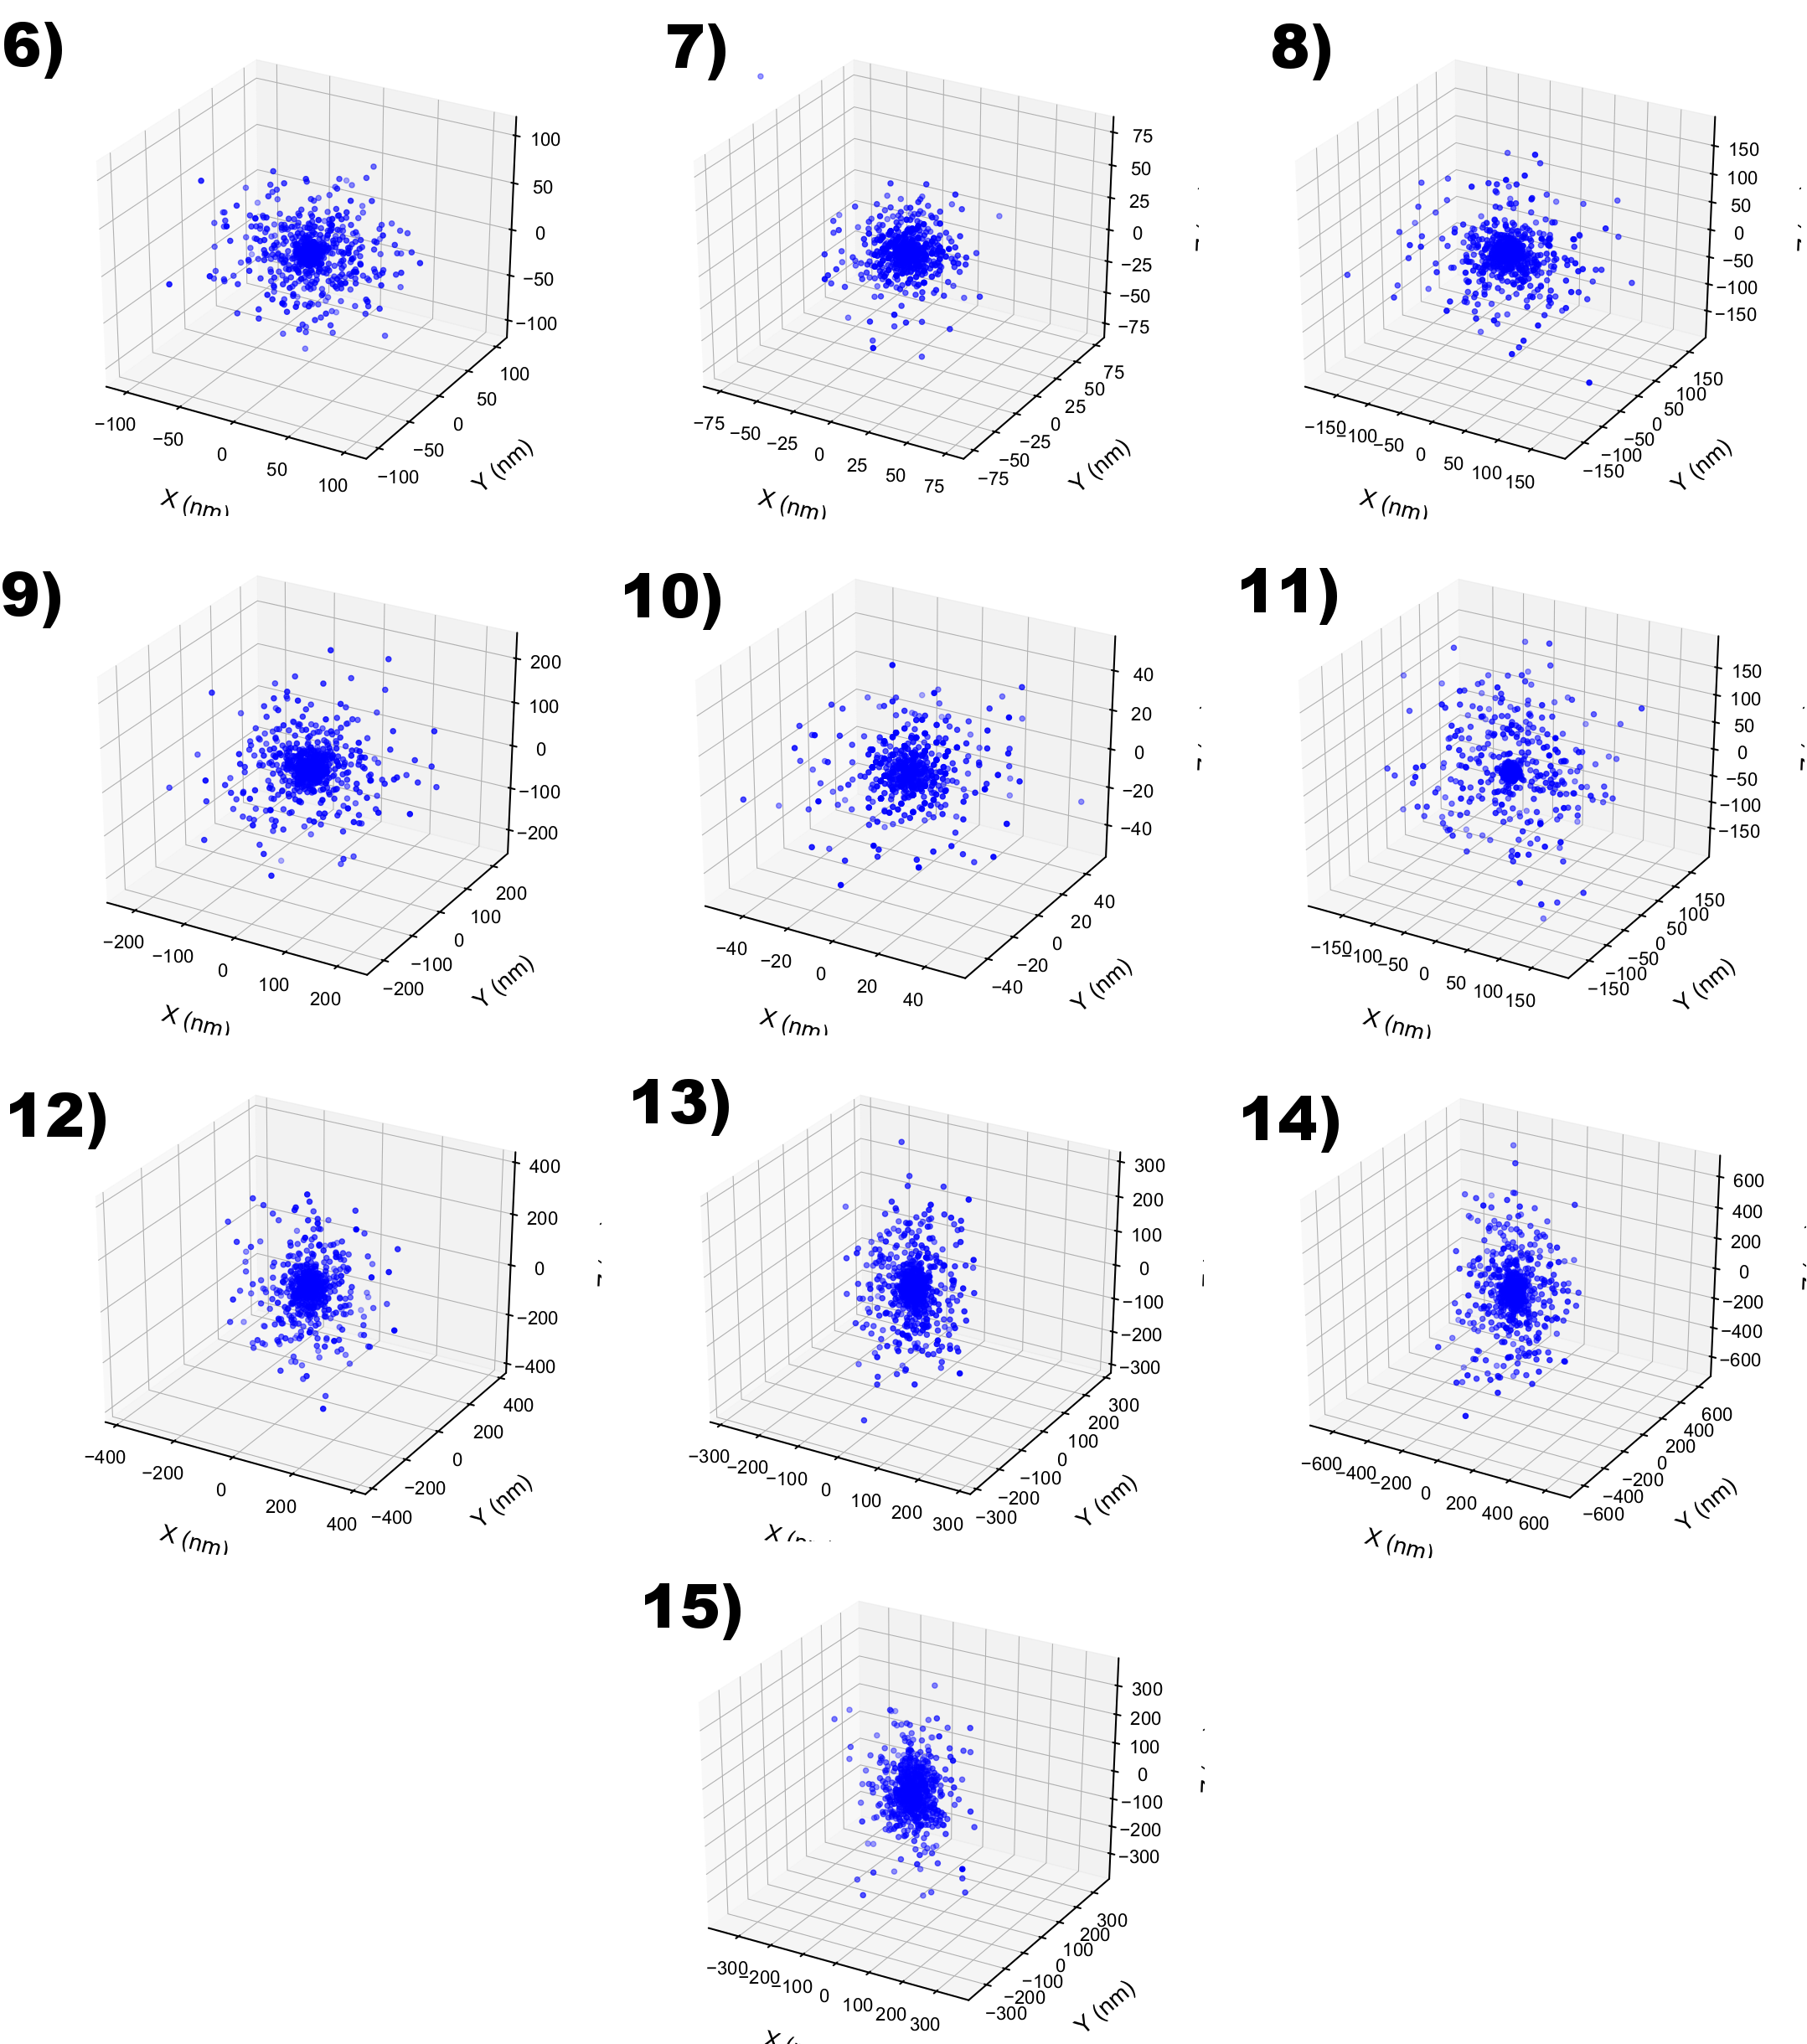
\includegraphics[width=\textwidth]{Figures/anisotropyHoleFrame.png}
    \caption{The periodic anisotropies of the carrier transport within the morphologies \textbf{6} - \textbf{15}.}
	\label{fig:MSD}
\end{figure}

\clearpage
\subsection{MSDs}


\begin{figure}[h!]\centering
	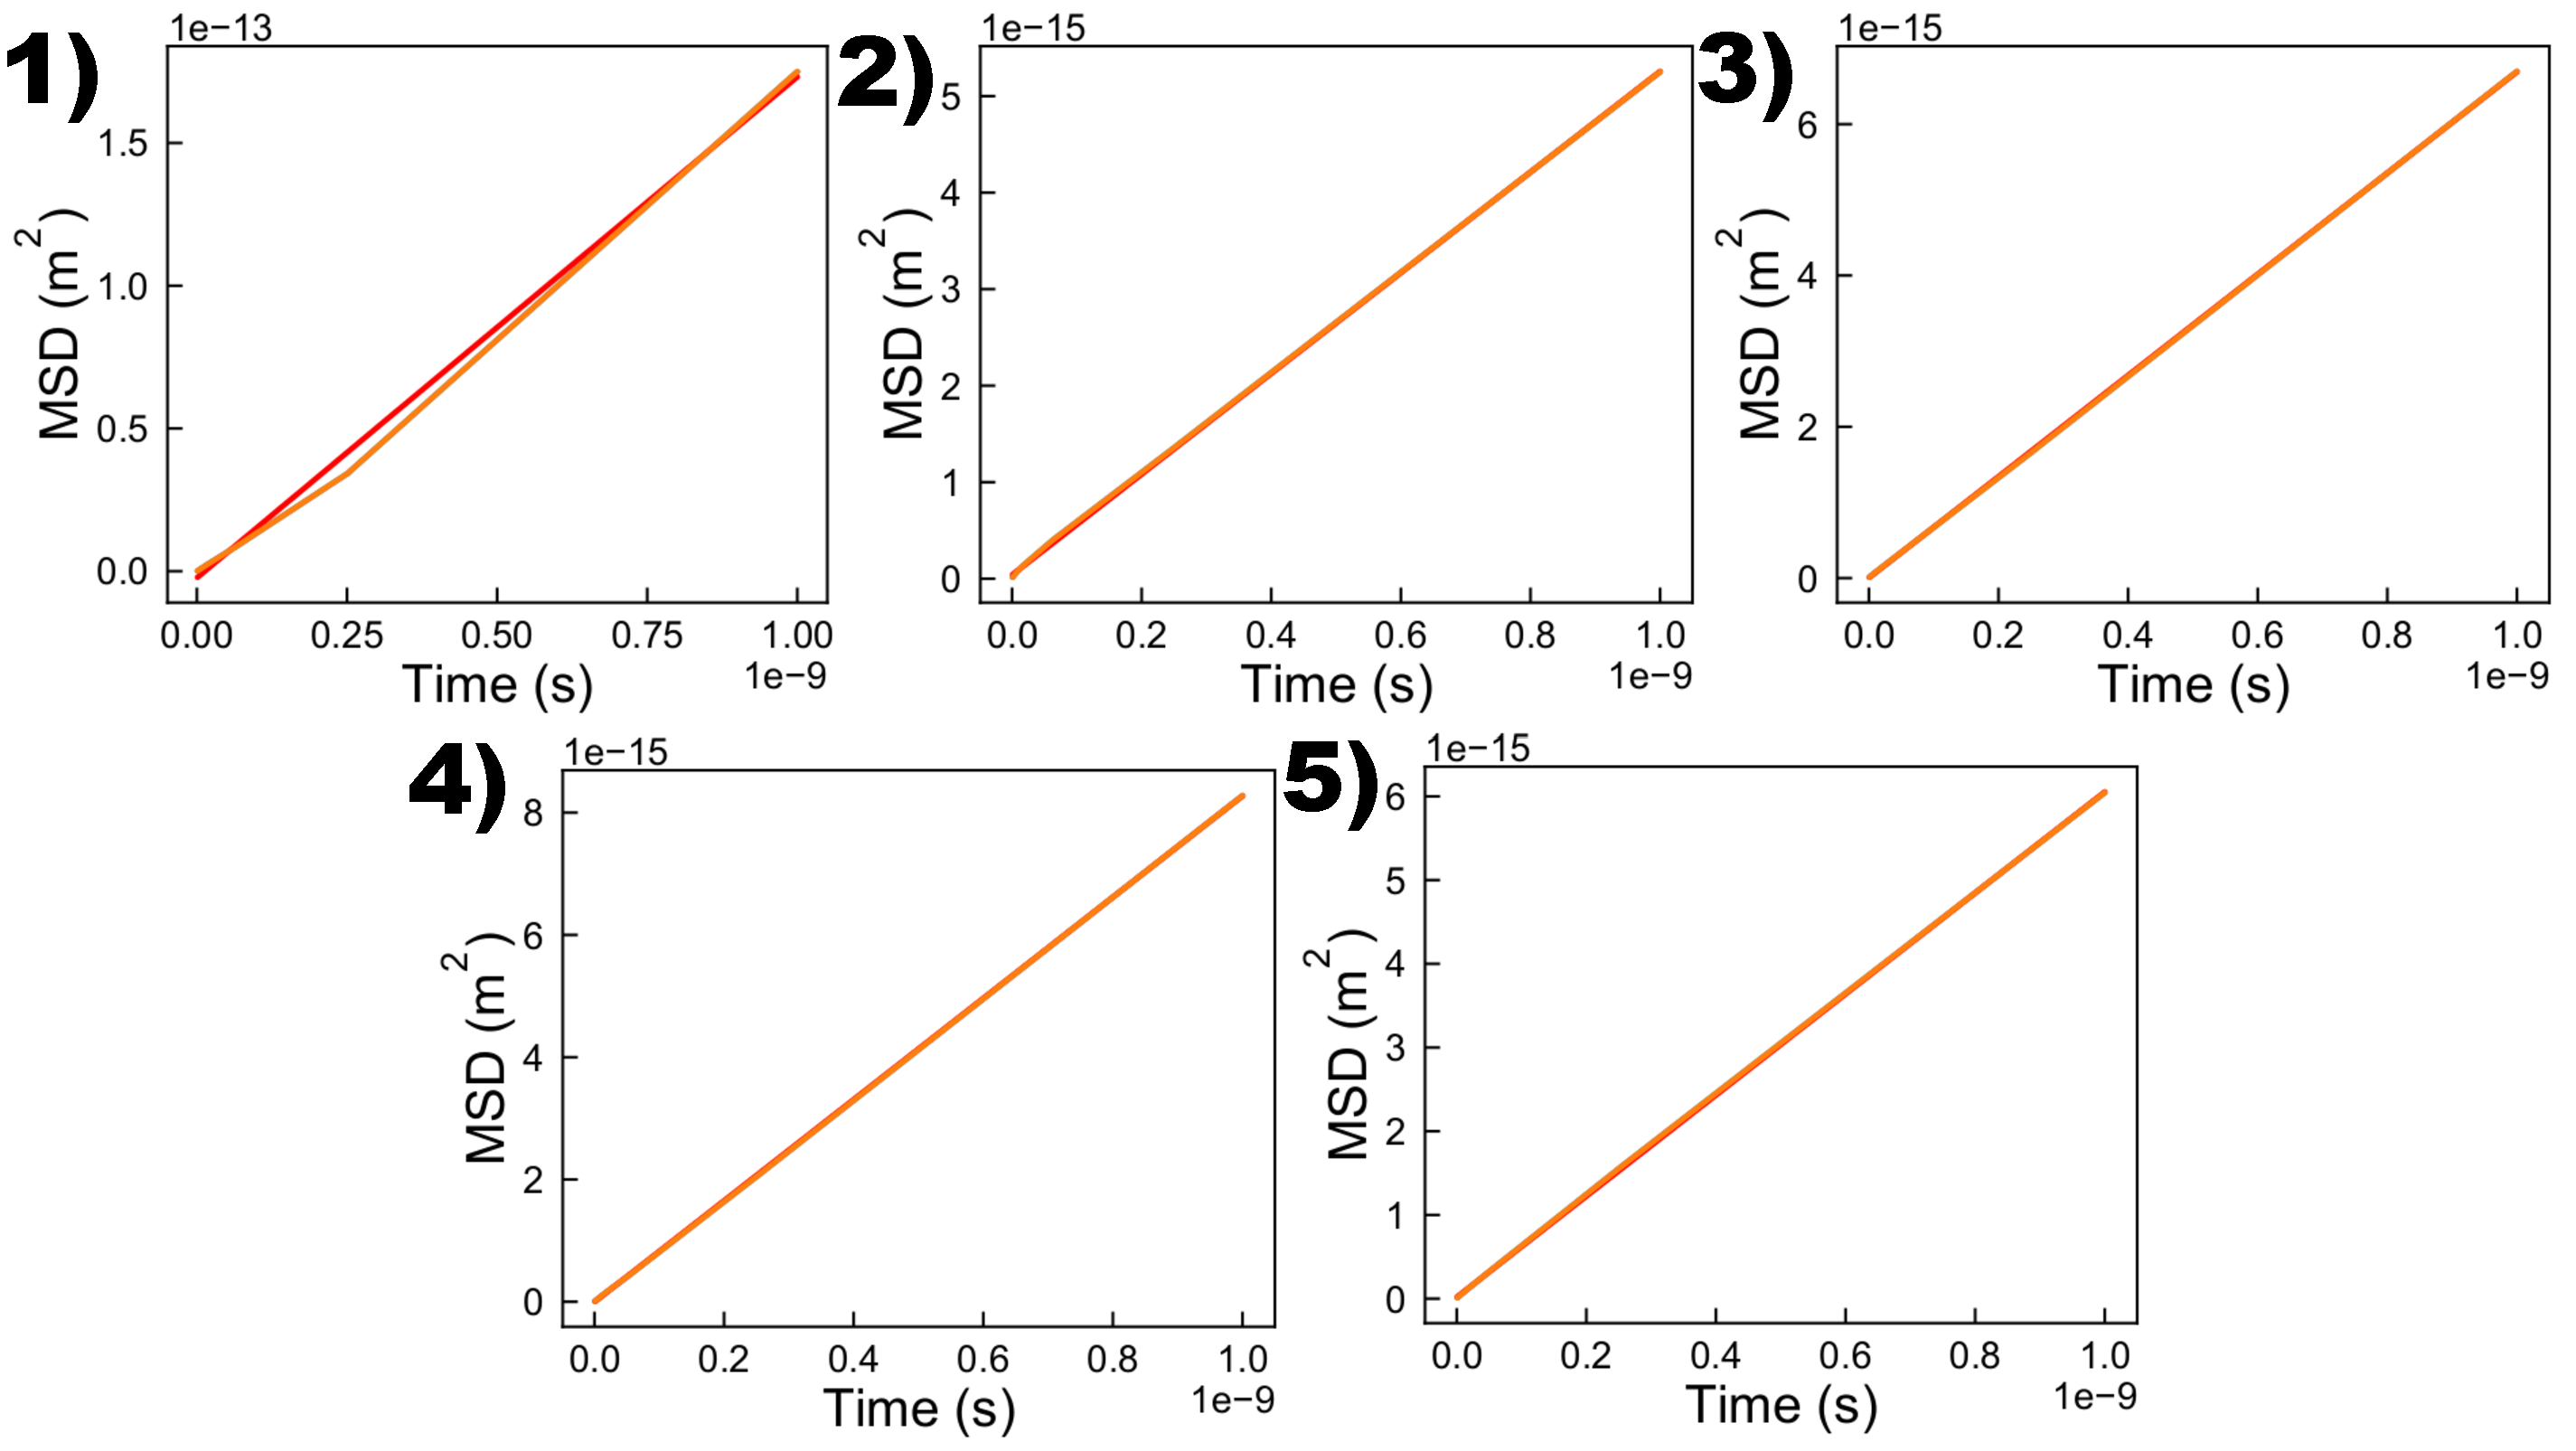
\includegraphics[width=\textwidth]{Figures/LinMSDHole.pdf}
    \caption{The linear mean squared displacement curves of the carriers within the morphologies \textbf{1} - \textbf{5}.}
	\label{fig:MSD}
\end{figure}


\clearpage
\subsection{Hopping Rate Distributions}

\begin{figure}[h!]\centering
    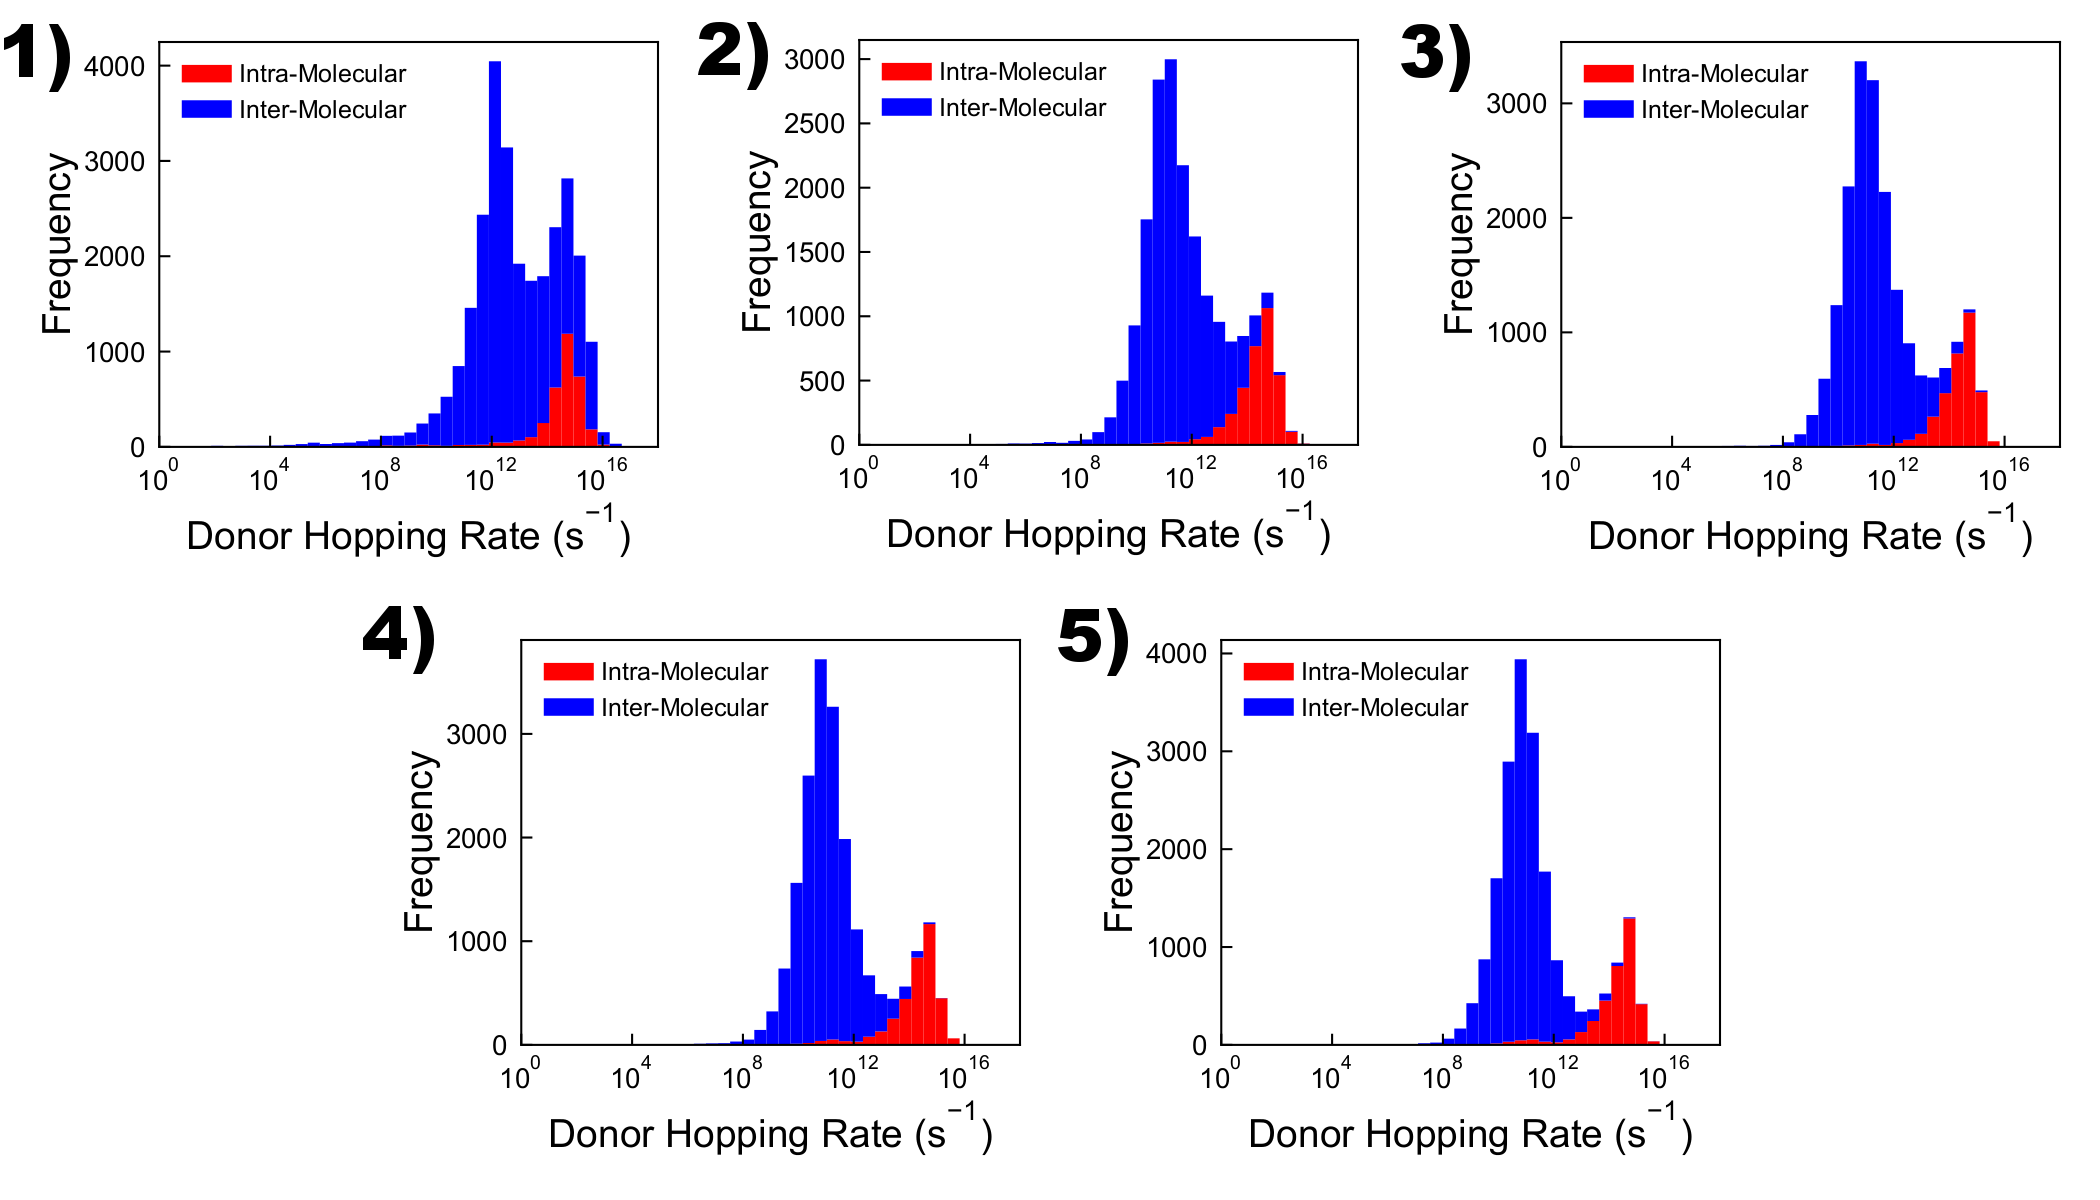
\includegraphics[width=\textwidth]{Figures/DonorHoppingRateMixed.png}
    \caption{The stacked hopping-rate distributions for intra- and inter-molecular hops executed by carriers within the morphologies \textbf{1} - \textbf{5}.}
	\label{fig:HoppingRateMixed}
\end{figure}

\clearpage


\bibliography{refs}
\bibliographystyle{unsrt}


\end{document}
